\documentclass[11pt]{article}
\textwidth 7in
\textheight 10in
\oddsidemargin -.25in
\evensidemargin -.25in
\topmargin -1in    
\usepackage{graphics}        
\usepackage{graphicx}
\usepackage{pifont}
\usepackage{amsmath,amsthm,amscd,amssymb,amsfonts}
\usepackage{latexsym}
\usepackage{upref}
\usepackage{color}
\begin{document}
\newcommand{\dsp}{\displaystyle}
\newcommand{\ihat}{{\bf{i}}}
\newcommand{\jhat}{{\bf{j}}}
\newcommand{\khat}{{\bf{k}}}
\newcommand{\Fhat}{{\bf{F}}}
\newcommand{\myyellow}{\colorbox[cmyk]{0,0,.15,0}}
\newcommand{\mygreen}{\colorbox[cmyk]{.05,0,.05,0}}
\newcommand{\mygrey}{\colorbox[cmyk]{0,0,0,.1}}
\newcommand{\xsblank}{\underline{\ \ \ \ \ \ \ }}
\newcommand{\smblank}{\underline{\ \ \ \ \ \ \ \ \ \ \ \ \ }}
\newcommand{\mdblank}{\underline{\ \ \ \ \ \ \ \ \ \ \ \ \ \ \ \ \ \ \ \ \ \ \ \ \ }}
\newcommand{\lgblank}{\underline{\ \ \ \ \ \ \ \ \ \ \ \ \ \ \ \ \ \ \ \ \ \ \ \ \ \ \ \ \ \ \ \ \ \ \ \ \ \ \ \ }}
\newcommand{\xlblank}{\underline{\ \ \ \ \ \ \ \ \ \ \ \ \ \ \ \ \ \ \ \ \ \ \ \ \ \ \ \ \ \ \ \ \ \ \ \ \ \ \ \ \ \ \ \ \ \ \ \ \ \ \ \ \ \ \ }}
\newcommand{\one }{\Large \ding{192}\normalsize}
\newcommand{\two }{\Large \ding{193}\normalsize}
\newcommand{\three}{\Large \ding{194}\normalsize}
\newcommand{\four}{\Large \ding{195}\normalsize}
\newcommand{\five}{\Large \ding{196}\normalsize}
%\pagestyle{headings}
%\markright{MATH 1120 Lab Worksheet \#1}
\thispagestyle{empty}

\noindent
\sffamily
\begin{center}
\huge 3.2:  Quadratic Equations, Functions, Zeros, and Models\normalsize

\rule{7in}{2pt}
\end{center}

\noindent \underline{\textbf{Quadratic Equations and Functions}}\\[.15in]
A \underline{quadratic equation} is an equation of the form \lgblank, where $a\ne 0$, and $a, b, c \in \mathbb{R}$. \\[.15in]
A \underline{quadratic function} is a function of the form \lgblank, where $a\ne 0$, and $a, b, c \in \mathbb{R}$. \\[.15in]
Solving a quadratic equation is equivalent to finding the zeros of a quadratic function. \\[.15in]
\framebox{
\begin{tabular}{p{1in}|c|c|c}
\textbf{Graphs:} &
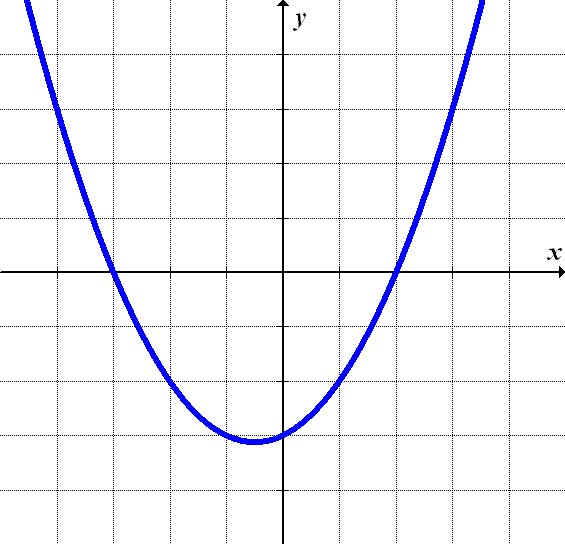
\includegraphics[width=1.75in]{parabola2.png} &
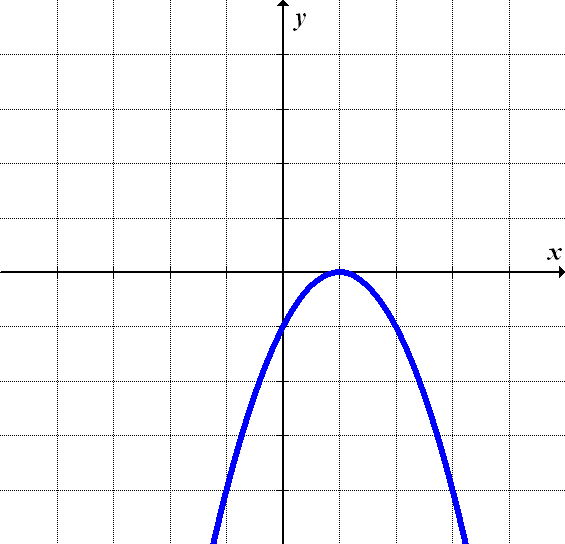
\includegraphics[width=1.75in]{parabola1.png} &
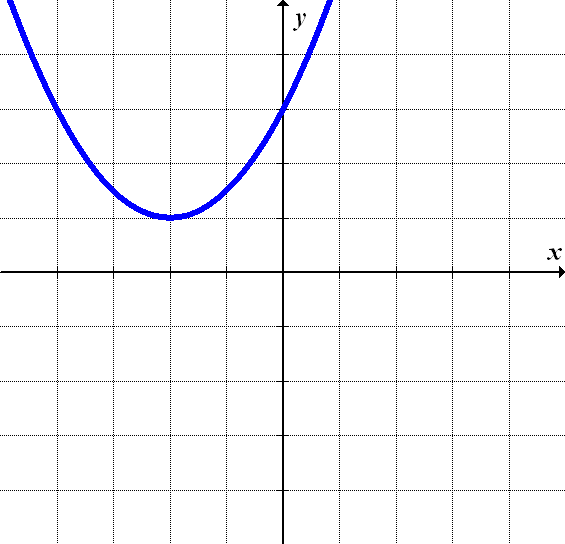
\includegraphics[width=1.75in]{parabola0.png} \\ \hline 
& & & \\[-.1in]
\textbf{\# of $x$-int:} & & & \\ \hline
& & & \\[-.1in]
\textbf{\# of zeros:} & & & \\ \hline
& & & \\[-.1in]
\textbf{Discriminant:} & & & \\ \hline
 & & & \\[-.1in]
\textbf{Solutions:} & & & \\
\end{tabular}}

\vspace{.15in}

\noindent \mygrey{
\begin{tabular}{p{7in}}
\textbf{(EX)}  Determine the nature of the solutions of the equation:\\[.15in]
\begin{tabular}{p{3.5in}p{3.5in}}
(a) $x^2-2x+4=0$ &
(b) $5t^2-7t=0$ \\[.5in]
\end{tabular}
\end{tabular}}

\vspace{.15in}

\noindent \underline{\textbf{Solving Quadratic Equations:}}  We will employ three methods for solving quadratic equations:
\begin{enumerate}
\item FACTORING

\vspace{.15in}
\noindent \mygrey{
\begin{tabular}{p{6.5in}}
\textbf{(EX)}  Solve by factoring:\\[.15in]
(a) $5t^2-7t=0$ \\[.75in]
(b) $3x^2+x-2=0$ \\[.75in]
(c) $x^2+4x=-4$\\[.75in]
\end{tabular}}

\newpage
\thispagestyle{empty}
\item COMPLETING THE SQUARE

Recall that $(x+A)^2 = x^2 + 2Ax + A^2$ is a perfect square trinomial.  Suppose we have an expression such as $x^2+18x$, and we want to add a constant so that it creates a perfect square:

$$x^2+18x+\xsblank = (\smblank)^2$$

\vspace{.15in}
\noindent \mygrey{
\begin{tabular}{p{6.5in}}
\textbf{(EX)}  Solve by completing the square:\\[.15in]
(a) $x^2-4x+2=0$ \\[1in]
(b) $t^2+3t-7=0$ \\[1in]
(c) $3x^2-6x-4=0$\\[1in]
(d) $2z^2+3z-2=0$\\[1in]
\end{tabular}}

\item THE QUADRATIC FORMULA (developed by completing the square on $ax^2+bx+c=0$)\\[.25in]
$$x=\lgblank$$

\vspace{.15in}
\noindent \mygrey{
\begin{tabular}{p{6.5in}}
\textbf{(EX)}  Solve using the quadratic formula:\\[.15in]
(a) $x^2-4x+2=0$ \\[.75in]
(b) $2z^2+3z-2=0$ \\[.75in]
\end{tabular}}

\end{enumerate}

\newpage
\thispagestyle{empty}

\noindent \underline{\textbf{Equations Reducible to Quadratic}}\\[.15in]
\noindent \mygrey{
\begin{tabular}{p{7in}}
\textbf{(EX)}  Solve:\\[.15in]
(a) $2x^4-9x^2=-4$ \\[1.5in]
(b) $x-8\sqrt{x}-9=0$ \\[1.5in]
(c) Find the zeros of the function:  $f(x) = x^{2/3} +3x^{1/3}-10$\\[1.5in]
(d) $2(t+2)^2-5(t+2)-12=0$\\[1.5in]
\end{tabular}}

\vspace{.15in}
\noindent \mygrey{
\begin{tabular}{p{7in}}
\textbf{(EX)}  The diagonal of a TV set is 30 inches long.  Its length is 12 inches less than twice the height.  Find the dimensions of the TV set.  \\[1.75in]
\end{tabular}}

\end{document}



